\section{Testgetriebene Entwicklung}
Testgetriebene Entwicklung, im Englischen Test-Driven-Development (TDD) wurde erstmalig von Kent Beck 2003 im Detail erläutert. Zuvor war die Technik "`Test-First"' aber schon seit 1999 im Kontext von Extreme Programming (XP) bekannt.
%TODO Quelle: "Extreme Programming". Computerworld. Retrieved January 11, 2011.
%TODO Quelle: Beck, K. Test-Driven Development by Example, Addison Wesley, 2003
Damit wurde aus der Entwicklungs-Methode "`Test-First"' ein Software-Entwicklungsprozess. 

Im Folgenden werde ich diesen Prozess näher beleuchten und am Beispiel von Ruby on Rails typische Testwerkzeuge aufzeigen. 
\subsection{Motivation}
  Das Erstellen einer gut abdeckenden Test-Suite für ein jedes größeres Softwareprojekt ist eine wichtige Vorraussetzungen um interne Qualitäten, wie Wartbarkeit und Zuverlässigkeit zu aktivieren. TDD soll nicht dazu dienen, die Software zu verifizieren. Dies ist aber ein positiver Nebeneffekt. Das Hauptziel ist es, den Code in Einklang mit dem Test zu schreiben, so dass der Test den Code antreibt (Test drives thes code). Der messbare Effekt davon, ist ein gut-testbarer Code, welcher in der Regel auch ein gut-wartbarer und verständlicher Code ist. Bad-Smells, wie God-Methode und geringe Kohäsion, werden schon im Keim erstickt werden, da diese nur äußerst schwer zu testen sind.

  \paragraph{Psychologische Aspekte und Aspekte des Projektmanagements}
  
  Kent Beck beschreibt die Hauptmotivation für TDD, als das "`managing fear during programming"' Management von Angst. So hat Angst verschiedene Auswirkungen auf die Entwicklung. Sie mache zögerlich, führe zu weniger Kommunikation und Feedback und mache den Programmierer "`mürrisch"' \citep[S. xi]{beck_test_2002}.
  
  %Die Motivation für die Wahl von Test-getriebener Entwicklung als primäre Entwicklungsstrategie wird mit dem
  
  Falls TDD die Fehlerdichte signifikant verringern würde und nur Code entstünde, der getestet wurde, so hätte dies auch soziale Auswirkungen auf das Entwicklerteam \citep[S. x]{beck_test_2002}. 
  \begin{enumerate}
   \item Die Qualitätssicherung könnte von einer reaktiven, auf eine proaktive Arbeit umstellen.
   \item Der Projektmanager kann den Ablauf der Entwicklung besser planen, da weniger überraschende Regressionsfehler im Laufe der Entwicklung auftreten
   \item Durch eine niedrige Fehlerdichte kann die Kontinuierliche Integration (Continuos Integration) möglich gemacht werden, und so der Kunde in den Entwicklungsprozess einbezogen werden
  \end{enumerate}
 
  TDD hat auch eine psychologische Motivation für den individuellen Programmierer.
  TDD fördert die Entwicklung in kleinen Schritten, und ermöglicht durch bestande Tests kleine "`Belohnungen"' für den Programmierer. Dadurch ist es leichter einen gewissen Arbeitsrhythmus zu erhalten, was stellenweise dem "`Flow"'\footnote{Schaffen-, Tätigkeitssrausch}  ähnelt oder diesen strukturiert ergänzen kann \citep{roger_brown_test_2008}.
  
\subsection{Ablauf}
  Ziel ist es, vor der Implementation eines Codes, einen Unittest zu implementieren. Davon ausgehend soll der geringstmögliche Code implementiert werden, damit der Test besteht. Zum Schluss wird refaktorisiert, bei TDD auch als Designphase genutzt.
  
  \begin{figure}[htbp]
 \centering
 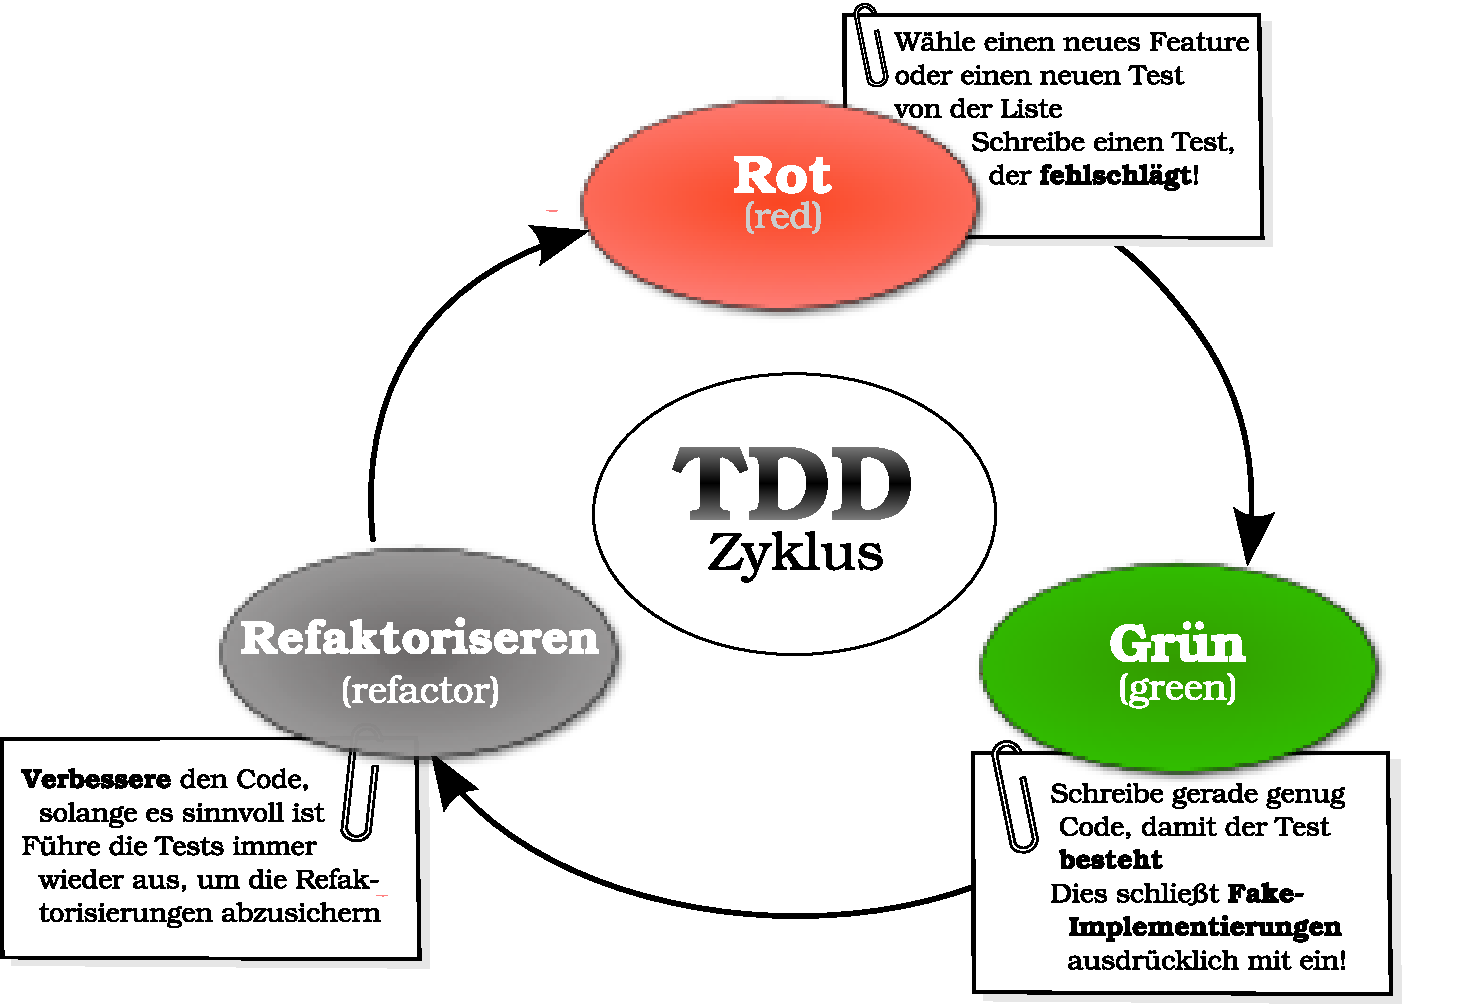
\includegraphics[width=0.85\textwidth]{./diagrams/red-green-refactor.pdf}
 % red-green-refactor.png: 884x602 pixel, 90dpi, 24.95x16.99 cm, bb=
 \caption{Red-Green-Refactor: Der TDD Entwicklungszyklus}
 
 \imgsource{Bildquelle: Der Autor}
 \label{fig:redgreenrefactor}
\end{figure}
  Im Detail sind das also folgende Phasen, vgl. Abbildung \ref{fig:redgreenrefactor}:
  \begin{enumerate}
   \item Schreibe einen neuen Test. Dies kann der erste eines neuen Features sein, oder aber ein Test, um Funktionalität zum aktuellen Feature hinzuzufügen
   \item Red: Führe alle Tests aus, um sicherzugehen, dass der Test fehlschlägt. Andernfalls ist der Test überflüssig.
   \item Green: Nachdem der Test fehlschlägt, implementiere nun den einfachsten Code, damit der Test besteht\\
   Dies kann ausdrücklich auch eine Fake-Implementierung sein, also z.B. die Rückgabe eines konstanten Wertes anstelle einer Berechnung. Wichtig ist, dass diese Phase so schnell wie möglich verlassen wird.
   \item Refactor: Nachdem der Test bestanden wird, folgt nun die \textbf{wichtigste Phase}, die Refaktorisierungsphase.\\
   Da wir bereits einen Test haben, der unser gewünschtes Systemverhalten widerspiegelt, können wir gefahrlos refaktorisieren, d.h. meist Duplikation eleminieren. In dieser Phase findet das Design des Codes statt. Man macht sich Gedanken, wie die vorhanden Klassen optimal refaktorisieren können, um Code-Smells zu eleminieren, und welches Entwurfsmuster angewendet werden kann.
  \end{enumerate}
  
  Jeder Unittest soll prinzipiell nur eine Eigenschaft testen, die Entwicklung erfolgt also in kleinen Schritten. Dies hat direkte Auswirkungen auf die zu entwickelnden Objekte und Methoden, die ebenfalls übersichtlich werden sollen, und somit dem Funktionsbegriff, eine Methode für eine Aufgabe und erweitert eine Klasse für eine Aufgabe, gerecht werden.
  
  Das ganze lässt sich auch in den übergeordneten Prozess zum Entwickeln eines Features einordnen.
  %RSPEC Buch macht das vor, Noch mal schauen, evtl alles Käse was ich hier geschrieben habe
  \begin{enumerate}
   \item Schreibe einen Integrations/Akzeptanztest um das aktuelle Feature zu implementieren
   \item Nach einer möglichen Überlegungs und Analysezeit, kann nun mit dem Implementierung der Teilschritt nach TDD Ablauf von oben verfahren werden
   \item Nachdem die Teilschritte implementiert wurden, kann nun mit dem Erfüllen des Akzeptanztests fortgefahren werden
  \end{enumerate}
  
  Somit werden 2 Testebenen erstellt, die Akzeptanz- und die Unittests.

  Im Prinzip soll jeder Änderung der Programmlogik ein fehlgeschlagener Test vorausgehen. Auch bei der Behebung von Defekten, also dem Bugfixing, soll zuerst ein Test geschrieben werden, der genau das Verhalten des Bugs widerspiegelt, und erst dann gefixt werden.
  
    
  \subsection{Mocks und Stubs}
  Beim Testen im Allgemeinen und bei TDD im Besonderen wird das Testen durch externe Abhängigkeiten erschwert. Dies können z.B. Klassen sein, die noch gar nicht implementiert wurden, externe Ressourcen (Netzwerkzugriffe, Versenden von Mails) oder externe Prozessen (Bezahlen in einem Onlineshop) sein. In diesen Situationen ist es angebracht, auf sogenannte Mocks und Stubs zurückzugreifen.
  
  Ein Stub ist eine nachahmende Funktion oder Objekt, welches die schwer zu isolierende Klasse während des Testfalls ersetzt. Im Beispiel ein Bezahlprozess einer Bestellung.
  \begin{lstlisting}
def test_report_failed_payment
  Payment.stubs(:pay).returns(false)
  
  bestellung = Bestellung.new()
  bestellung.commit()
  
  assert bestellung.errors.present?
end


  \end{lstlisting}
  Mit dem oben angegeben (Pseudo) Rubycode würde man z.B. mittels des Mock-Frameworks mocha ein Mockobjekt erzeugen, welches den (Fantasie-) Bezahlprozess nachahmt, und die Methode "`pay"' ersetzt, so dass sie immer "`false"' zurückgibt.
  So kann z.B. das Objekt Bestellung gefahrlos Bezahlungen auslösen. Der genaue Ablauf innerhalb des Bezahlprozesses ist die Bestellung unwichtig, lediglich der Rückgabewert, ob die Bezahlung erfolgreich war oder nicht.
  
  Als Ergänzung dazu gibt es Mocks. Ähnlich wie die Stubs ersetzen sie Methoden oder Objekte, um statt komplexer Operationen fixe Werte zurückzugeben. Zusätzlich dienen Mocks selbst als Testfall. Ein Mock wartet darauf, ob die Methode, wie sie definiert wurde, auch tatsächlich aufgerufen wurde.
  
  Hier z.B. ein Mock, um statt des heutigen Datums das von vor einer Woche zurückzugeben
  \begin{lstlisting}
def test_always_fail
  Date.mocks(:today).returns( 7.days.ago)
end
  \end{lstlisting}
  Der gezeigte Programmcode wird jedesmal fehlschlagen, da von einem Mock erwartet wird, dass er während des Tests genau einmal aufgerufen wird. Ist dies nicht der Fall, gilt der Test als nicht bestanden. Mocks fungieren somit als zusätzliche Möglichkeit Interna des Programmflusses zu testen. 


  
  \subsection{Vorteile von TDD}
   
  Die Test-Suite, die durch TDD entsteht, kann als zusätzliche Dokumentation dienen, die nie veraltet, im Gegensatz zu einer geschriebenen Dokumentation \citep{palermo_guidelines_2006}.
  
  Die Software-Engineering Literatur ist sich einig, dass ein Bug teurer wird, je später er gefunden wird \citep{hunt_pragmatic_1999}[S. 238]. TDD hilft somit, einen Bug so frühzeitig wie möglich zu entdecken, und hat so das Potenzial, Budget einzusparen.
  
  Softwaresysteme, die durch TDD entstehen, tendieren dazu deutlich besser designt, lose gekoppelt und besser wartbar zu sein \citep{beck_test_2002} \citep{palermo_guidelines_2006}, da Refaktorisierungen mit hoher Zuversicht durchgeführt werden können
  
  Zusammenfassend führt TDD zu einer erhöhten Produktivität, da das Maß an manuellen Tests reduziert wird und Debuggen deutlich weniger wird \citep{palermo_guidelines_2006}.
  
  \subsection{Nachteile und Grenzen von TDD}
  Es gibt bestimmte Programmieraufgaben, die nicht allein durch die testgetriebene Entwicklung implementiert werden können. So seinen Nebenläufigkeit oder Software Sicherheit genannt, in denen TDD als Zielgeber nicht ausreiche \citep[S. xii]{beck_test_2002}.
  
  Zudem stelle die Testgetriebene Entwicklung kein Ersatz für andere Arten von Tests, wie Performanz/Stress und Usability-Test \citep[S. 86]{beck_test_2002}.
  \subsection{Behavior Driven Development}
  
  Eine oft erwähnte Variante von TDD ist die Verhaltensgetriebene Entwicklung (Behavior-Driven-Development -- BDD). Dabei dienen hier Akzeptanztests als treibende Kraft der Entwicklung. Diese beschreiben ein Verhalten (Behavior). Der Fokus liegt also nicht auf Implementationsdetails, sondern soll, in einer domainspezifischen Sprache, das Verhalten und die daraus resultierenden Erwartungen des Systems beschreiben.
  
  Dies drückt sich meist auch in dem Vokabular aus. Während bei klassischen Unit-Tests, und damit auch bei TDD, die Begriffsdomain  "`Zusicherungen"' (assertions) und "`Tests"' beinhaltet, so hat BDD stattdessen "`Erwartungen"' (expectations) und "`Spezifikationen"' (specs/specifiations), und verwendet oft das Modalverb "`sollte"' (should).
  
  \subsection{Design Driven Testing}
  Design Driven Testing soll eine Umkehrung von Testgetriebener Software sein und wird Stephens und Rosenberg als Alternative dazu vorgeschlagen \citep{stephens_design_2010}. Sie kritisieren, dass TDD in Reinform betrieben, lediglich Unittests, aber keine Dokumentation oder höhere Tests höherer Levels produziert. Weiterhin monieren sie, dass TDD zu schwierig und aufwändig sei. Sie schlagen vor, stattdessen die Tests durch das Software-Design steuern zu lassen und sich auf komplexe Code-Abschnitte zu konzentrieren, anstatt wirklich jeden Code durch einen vorausgegangen Test entstehen zu lassen. Sie proklamieren die Nutzung von Akzeptanz- anstelle der Unittests. Code-Qualität soll durch ein gründliches vorheriges Design anstelle nachträglicher massiver Refaktorisierungen bewerkstelligt werden.
  DDT eignet sich für größere Teams, da Wert auf manuelle Tests gelegt wird und z.B. ein QA-Team eingebunden wird.